\documentclass[12pt,a4paper]{article}

% ─── Page Layout ───────────────────────────────────────────────────────────────
\usepackage[a4paper, margin=0.8in, headheight=14pt]{geometry}

% ─── Fonts (XeLaTeX) ───────────────────────────────────────────────────────────
\usepackage{fontspec}
\usepackage{unicode-math}
\setmainfont{TeX Gyre Pagella}
\setmonofont[Scale=0.88]{TeX Gyre Cursor}
\setmathfont{Latin Modern Math}

% ─── Packages ──────────────────────────────────────────────────────────────────
\usepackage{xcolor}
\usepackage{colortbl}
\usepackage{titlesec}
\usepackage{enumitem}
\usepackage{tabularx}
\usepackage{longtable}
\usepackage{booktabs}
\usepackage{array}
\usepackage{amsmath}
\usepackage{tikz}
\usetikzlibrary{shapes.geometric, arrows.meta, positioning, calc, fit, decorations.pathreplacing, patterns}
\usepackage{tcolorbox}
\tcbuselibrary{skins, breakable}
\usepackage{hyperref}
\usepackage{fancyhdr}
\usepackage{graphicx}
\usepackage{microtype}
\hyphenpenalty=10000
\exhyphenpenalty=10000
\sloppy
\usepackage{caption}
\usepackage{setspace}
\usepackage{multirow}
\usepackage{tocloft}

% ─── Q&A helper ────────────────────────────────────────────────────────────────
\newcommand{\Q}[1]{\textbf{#1}\par\noindent\ignorespaces}

% ─── Colour Palette ────────────────────────────────────────────────────────────
\definecolor{myred}{RGB}{196,30,58}
\definecolor{mydark}{RGB}{30,30,50}
\definecolor{mygreen}{RGB}{14,120,80}
\definecolor{myteal}{RGB}{0,130,140}
\definecolor{myamber}{RGB}{180,100,0}
\definecolor{mypurple}{RGB}{100,30,160}
\definecolor{mygray}{RGB}{246,247,249}
\definecolor{mgframe}{RGB}{180,185,200}
\definecolor{watermark}{RGB}{145,150,170}
\definecolor{hdrred}{RGB}{250,232,235}
\definecolor{hdrgreen}{RGB}{220,244,233}
\definecolor{hdrteal}{RGB}{220,242,244}
\definecolor{hdramber}{RGB}{253,242,215}
\definecolor{hdrpurple}{RGB}{238,228,255}
\definecolor{hdrgray}{RGB}{238,240,245}

% ─── Section Formatting ────────────────────────────────────────────────────────
\titleformat{\section}
  {\large\bfseries\color{myred}}{\thesection.}{0.5em}{}
  [\vspace{1pt}{\color{myred}\rule{\linewidth}{0.8pt}}]
\titleformat{\subsection}
  {\normalsize\bfseries\color{myteal}}{\thesubsection}{0.5em}{}
\titlespacing*{\section}{0pt}{18pt}{7pt}
\titlespacing*{\subsection}{0pt}{11pt}{4pt}

% ─── Paragraph ─────────────────────────────────────────────────────────────────
\setlength{\parindent}{0pt}
\setlength{\parskip}{4pt}

% ─── TOC Styling ───────────────────────────────────────────────────────────────
\renewcommand{\cfttoctitlefont}{\large\bfseries\color{myred}}
\renewcommand{\cftaftertoctitle}{\par\noindent{\color{myred}\rule{\linewidth}{0.8pt}}}
\setlength{\cftbeforetoctitleskip}{0pt}
\setlength{\cftaftertoctitleskip}{6pt}
\renewcommand{\cftsecfont}{\normalsize\bfseries\color{mydark}}
\renewcommand{\cftsecpagefont}{\normalsize\bfseries\color{mydark}}
\renewcommand{\cftsecleader}{\cftdotfill{\cftdotsep}}
\setlength{\cftbeforesecskip}{7pt}
\renewcommand{\cftsubsecfont}{\small\color{mydark}}
\renewcommand{\cftsubsecpagefont}{\small\color{mydark}}
\setlength{\cftbeforesubsecskip}{3pt}
\setlength{\cftsubsecindent}{1.4em}

% ─── Table helpers ─────────────────────────────────────────────────────────────
\renewcommand{\arraystretch}{1.45}
\setlength{\tabcolsep}{6pt}
\arrayrulecolor{mydark}
\newcolumntype{B}[1]{>{\small\bfseries\raggedright\arraybackslash}m{#1}}
\newcolumntype{Y}{>{\small\raggedright\arraybackslash}X}
\renewcommand{\tabularxcolumn}[1]{m{#1}}

% ─── Header / Footer ───────────────────────────────────────────────────────────
\pagestyle{fancy}
\fancyhf{}
\fancyhead[L]{\small\color{myred}\textbf{EC403}\;\color{mydark}--- Microprocessor and Microcontroller}
\fancyhead[R]{\small\color{myteal}\textbf{Module 1 Notes}}
\fancyfoot[C]{\small\color{mydark}\thepage}
\fancyfoot[R]{\small\color{watermark}\textit{\copyright\ Biraj Sarkar (CGEC)}}
\renewcommand{\headrulewidth}{0.5pt}
\renewcommand{\footrulewidth}{0.3pt}

% ─── Hyperref ──────────────────────────────────────────────────────────────────
\hypersetup{
  colorlinks=true, linkcolor=myteal, urlcolor=myteal,
  pdfauthor={Biraj Sarkar (CGEC)},
  pdftitle={EC403 --- Module 1 Notes: 8085 and 8086 Microprocessor Systems}
}

% ─── tcolorbox styles ──────────────────────────────────────────────────────────
\tcbset{
  tikzbox/.style={
    colback=mygray, colframe=mgframe, boxrule=0.6pt, arc=4pt,
    left=8pt, right=8pt, top=6pt, bottom=6pt,
    colbacktitle=mgframe, coltitle=mydark, fonttitle=\small\bfseries
  },
  defbox/.style={
    colback=hdrgreen, colframe=mygreen, boxrule=0.8pt, arc=4pt,
    left=9pt, right=9pt, top=6pt, bottom=6pt,
    colbacktitle=mygreen, coltitle=white, fonttitle=\small\bfseries
  },
  formulabox/.style={
    colback=hdrteal, colframe=myteal, boxrule=0.8pt, arc=4pt,
    left=9pt, right=9pt, top=7pt, bottom=7pt,
    colbacktitle=myteal, coltitle=white, fonttitle=\small\bfseries
  },
  examplebox/.style={
    colback=hdramber, colframe=myamber, boxrule=0.8pt, arc=4pt,
    left=9pt, right=9pt, top=6pt, bottom=6pt,
    colbacktitle=myamber, coltitle=white, fonttitle=\small\bfseries
  },
  masonbox/.style={
    colback=hdrpurple, colframe=mypurple, boxrule=0.8pt, arc=4pt,
    left=9pt, right=9pt, top=6pt, bottom=6pt,
    colbacktitle=mypurple, coltitle=white, fonttitle=\small\bfseries
  },
  exambox/.style={
    colback=hdrpurple, colframe=mypurple, boxrule=1pt, arc=5pt,
    left=10pt, right=10pt, top=8pt, bottom=8pt,
    colbacktitle=mypurple, coltitle=white, fonttitle=\bfseries,
    breakable, title after break={\textbf{Frequently Asked / Viva Questions (contd.)}}
  }
}
\tcbset{breakable}
\tcbset{after={\par\color{black}}}

% ─── TikZ styles ───────────────────────────────────────────────────────────────
\tikzset{
  block/.style={rectangle, draw=myteal, fill=hdrteal,
    text width=2.4cm, align=center, minimum height=0.95cm,
    font=\small, rounded corners=3pt, line width=0.7pt},
  redblock/.style={rectangle, draw=myred, fill=hdrred,
    text width=2.4cm, align=center, minimum height=0.95cm,
    font=\small, rounded corners=3pt, line width=0.7pt},
  amberblock/.style={rectangle, draw=myamber, fill=hdramber,
    text width=2.4cm, align=center, minimum height=0.95cm,
    font=\small, rounded corners=3pt, line width=0.7pt},
  sumjunc/.style={circle, draw=myamber, fill=hdramber,
    minimum size=0.62cm, font=\small, line width=0.8pt},
  arrow/.style={-Stealth, thick, color=mydark},
  redarrow/.style={-Stealth, thick, color=myred},
  line/.style={thick, color=mydark}
}

\begin{document}

% ─── Title Page ───────────────────────────────────────────────────────────────
\begin{center}
  {\LARGE\bfseries\color{myred} EC403 --- Microprocessor and Microcontroller}\\[5pt]
  {\normalsize\color{mydark} Semester IV \quad$\bullet$\quad 3L:0T:0P \quad$\bullet$\quad 3 Credits}\\[3pt]
  {\normalsize\color{myteal}\textbf{Module 1 Exam Notes: 8085 and 8086 Microprocessor Systems}}\\[3pt]
  {\small\color{mydark} CGEC \;$|$\; B.Tech ECE (2023--27) \;$|$\; \textit{Biraj Sarkar}}
\end{center}
\vspace{2pt}
\noindent{\color{myred}\rule{\linewidth}{1.5pt}}
\vspace{2pt}

\hypersetup{linkcolor=mydark}
\tableofcontents
\hypersetup{linkcolor=myteal}
\newpage

\section{Overview of Microcomputer Systems and Building Blocks}

\begin{tcolorbox}[defbox, title={Microprocessor, Microcomputer, and Microcontroller}]
A \textbf{microprocessor} is a multipurpose, programmable, clock-driven, register-based central processing unit (CPU) fabricated on a single integrated circuit chip. It fetches, decodes, and executes binary instructions from external memory.

A \textbf{microcomputer} is a complete functional computing system comprising a microprocessor, primary memory (ROM and RAM), clock and reset generation circuits, and input/output (I/O) peripheral interfaces interconnected via system buses.

A \textbf{microcontroller} is an integrated computer-on-a-chip containing a CPU, fixed memory, timer/counters, and I/O ports in a single silicon package.
\end{tcolorbox}

\begin{tcolorbox}[tikzbox, title={Microcomputer System Bus Architecture}]
\centering
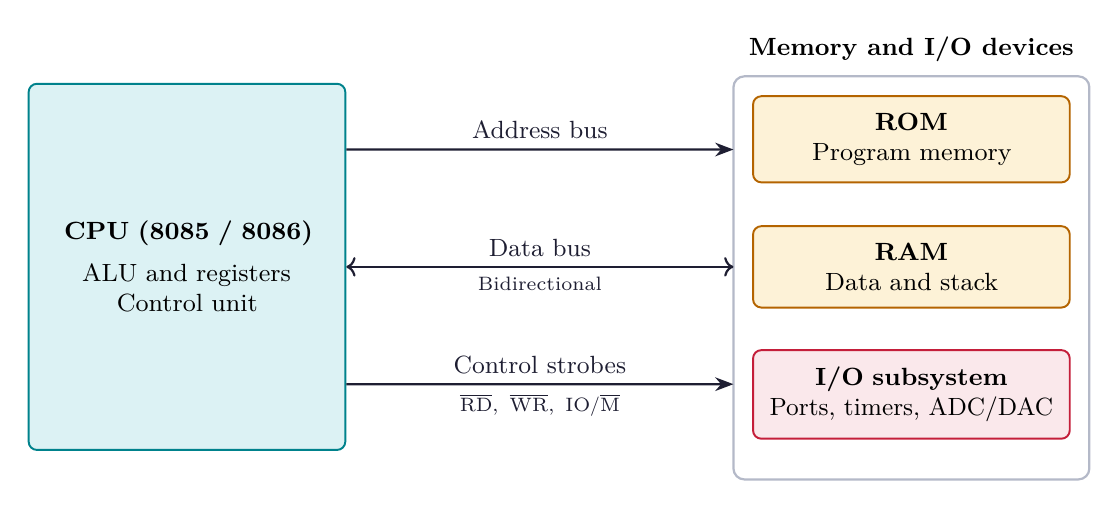
\begin{tikzpicture}[every node/.style={font=\small},
  unit/.style={align=center, inner sep=6pt, text width=3.6cm}]
  \node[block, unit, minimum height=4.65cm] (cpu) at (0,0)
    {\textbf{CPU (8085 / 8086)}\\[4pt] ALU and registers\\ Control unit};
  \node[amberblock, unit, minimum height=1.0cm] (rom) at (9.2,1.62)
    {\textbf{ROM}\\ Program memory};
  \node[amberblock, unit, minimum height=1.0cm] (ram) at (9.2,0)
    {\textbf{RAM}\\ Data and stack};
  \node[redblock, unit, minimum height=1.0cm] (io) at (9.2,-1.62)
    {\textbf{I/O subsystem}\\ Ports, timers, ADC/DAC};
  % Each arrow represents a distinct bus connected to the device group.
  \draw[mgframe,thick,rounded corners=4pt] (6.94,-2.7) rectangle (11.46,2.42);
  \node[above,font=\small\bfseries] at (9.2,2.48) {Memory and I/O devices};
  \draw[arrow,thick] ([yshift=1.49cm]cpu.east) --
    node[above] {Address bus} (6.94,1.49);
  \draw[arrow,<->,thick] (cpu.east) --
    node[above] {Data bus} node[below,font=\scriptsize] {Bidirectional} (6.94,0);
  \draw[arrow,thick] ([yshift=-1.49cm]cpu.east) --
    node[above] {Control strobes}
    node[below,font=\scriptsize] {$\overline{\mathrm{RD}},\ \overline{\mathrm{WR}},\ \mathrm{IO}/\overline{\mathrm M}$}
    (6.94,-1.49);
\end{tikzpicture}
\end{tcolorbox}

\subsection{Building Blocks and Bus Structures}
\begin{enumerate}[leftmargin=*]
  \item \textbf{Address Bus:} Unidirectional lines that specify the physical memory address or I/O port address. For an $n$-bit address bus, the addressable space is $2^n$ bytes (16 bits in 8085 $\to$ 64 KiB; 20 bits in 8086 $\to$ 1 MiB).
  \item \textbf{Data Bus:} Bidirectional lines that transfer instruction codes and data between the CPU and memory/peripherals (8 bits in 8085; 16 bits in 8086).
  \item \textbf{Control Bus:} Dedicated timing and status lines that identify and synchronize the active transfer cycle ($\overline{\mathrm{RD}}$, $\overline{\mathrm{WR}}$, $\mathrm{IO}/\overline{\mathrm{M}}$, $\mathrm{ALE}$, $\mathrm{READY}$).
  \item \textbf{Bus Buffering and Latching:}
  \begin{itemize}[leftmargin=*]
    \item \textbf{74LS373 (Octal D-type Transparent Latch):} Demultiplexes lower address bits from data lines ($AD_0-AD_7$) using the Address Latch Enable ($\mathrm{ALE}$) pulse.
    \item \textbf{74LS245 (Octal Bidirectional Bus Transceiver):} Enhances bus fan-out drive capacity and isolates system components. Direction is governed by $\mathrm{DIR}$ (driven by $\mathrm{DT}/\overline{\mathrm{R}}$) and active-low chip enable $\overline{\mathrm{OE}}$ (driven by $\overline{\mathrm{DEN}}$).
  \end{itemize}
\end{enumerate}

\section{Intel 8085 Microprocessor Architecture and Pin Details}

\begin{tcolorbox}[defbox, title={Intel 8085 Architectural Overview}]
The \textbf{Intel 8085A} is an 8-bit NMOS microprocessor operating on a single $+5\,\mathrm{V}$ DC supply. It has a multiplexed 8-bit data/lower address bus ($AD_0-AD_7$) and an 8-bit high address bus ($A_8-A_{15}$), addressing $64\,\mathrm{KiB}$ ($2^{16}$ bytes) of memory. It features an on-chip clock generator operating at an internal frequency of $3.072\,\mathrm{MHz}$ (using a $6.144\,\mathrm{MHz}$ quartz crystal connected across pins $X_1-X_2$).
\end{tcolorbox}

\begin{tcolorbox}[tikzbox, title={Intel 8085 Functional Internal Architecture}]
\centering
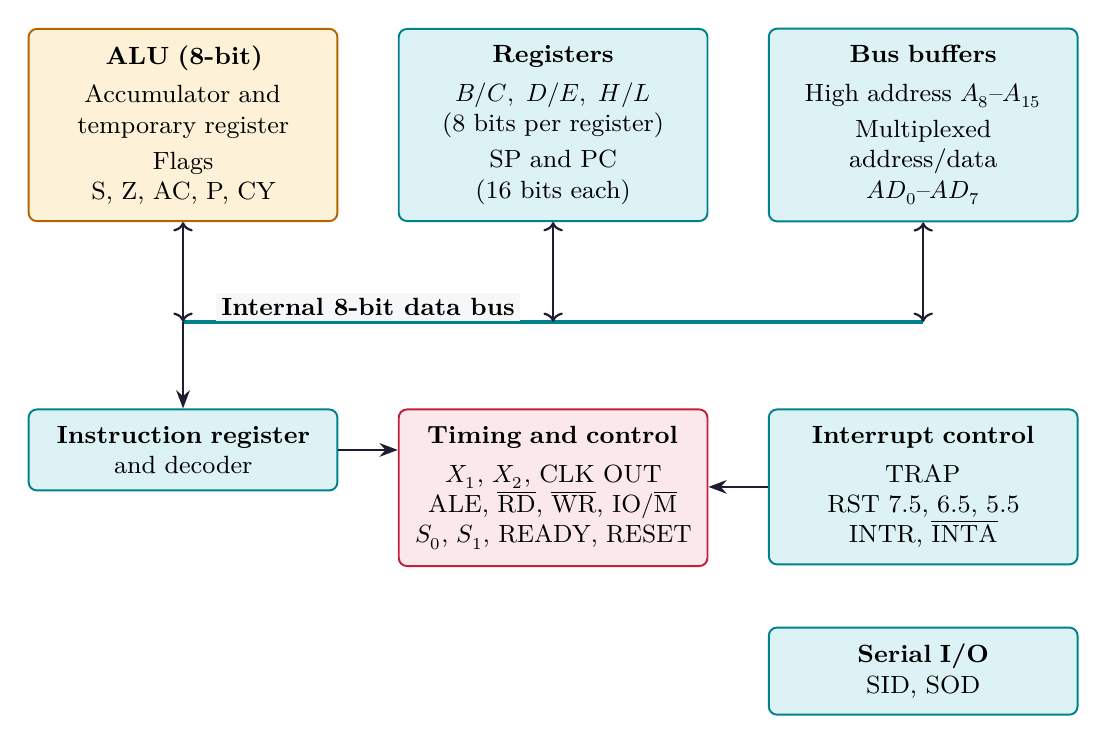
\begin{tikzpicture}[every node/.style={font=\small},
  unit/.style={align=center, text width=3.5cm, inner sep=6pt}]
  \node[amberblock,unit] (alu) at (0,2.75) {\textbf{ALU (8-bit)}\\[3pt]
    Accumulator and\\ temporary register\\[2pt] Flags\\S, Z, AC, P, CY};
  \node[block,unit] (regs) at (4.7,2.75) {\textbf{Registers}\\[3pt]
    $B/C,\ D/E,\ H/L$\\(8 bits per register)\\[2pt] SP and PC (16 bits each)};
  \node[block,unit] (buf) at (9.4,2.75) {\textbf{Bus buffers}\\[3pt]
    High address $A_8$--$A_{15}$\\[2pt] Multiplexed address/data\\ $AD_0$--$AD_7$};

  \draw[very thick,myteal] (0,0.25) -- (9.4,0.25);
  \node[above,font=\small\bfseries,fill=mygray,inner sep=2pt] at (2.35,0.25)
    {Internal 8-bit data bus};
  \foreach \unitname/\column in {alu/0,regs/4.7,buf/9.4}
    \draw[arrow,<->,thick] (\unitname.south) -- (\column,0.25);

  \node[block,unit,anchor=north] (decode) at (0,-0.85)
    {\textbf{Instruction register}\\ and decoder};
  \node[redblock,unit,anchor=north] (ctrl) at (4.7,-0.85)
    {\textbf{Timing and control}\\[3pt]
     $X_1$, $X_2$, CLK OUT\\
     ALE, $\overline{\mathrm{RD}}$, $\overline{\mathrm{WR}}$, $\mathrm{IO}/\overline{\mathrm M}$\\
     $S_0$, $S_1$, READY, RESET};
  \node[block,unit,anchor=north] (irq) at (9.4,-0.85)
    {\textbf{Interrupt control}\\[3pt] TRAP\\ RST 7.5, 6.5, 5.5\\ INTR, $\overline{\mathrm{INTA}}$};
  \node[block,unit,anchor=north] (serial) at (9.4,-3.62)
    {\textbf{Serial I/O}\\ SID, SOD};
  \draw[arrow,thick] (0,0.25) -- (decode.north);
  \draw[arrow,thick] (decode.east) -- (decode.east -| ctrl.west);
  \draw[arrow,thick] (irq.west) -- (irq.west -| ctrl.east);
\end{tikzpicture}
\end{tcolorbox}

\subsection{8085 Pin Description and Categorization}
\par\vspace{4pt}\noindent
\begingroup
\renewcommand{\arraystretch}{1.2}
\setlength{\extrarowheight}{1.5pt}
\begingroup
\setlength{\LTleft}{0pt}
\setlength{\LTright}{0pt}
\begin{longtable}{|B{2.8cm}|B{2.8cm}|>{\small\raggedright\arraybackslash}m{\dimexpr(\linewidth-2.8cm-2.8cm-6\tabcolsep-4\arrayrulewidth)/1\relax}|}
\hline
\textbf{Functional Group} & \textbf{Pin Names} & \textbf{Pin Function and Operating Characteristics} \\ \hline
\endfirsthead
\hline
\textbf{Functional Group} & \textbf{Pin Names} & \textbf{Pin Function and Operating Characteristics} \\ \hline
\endhead
Address \& Data & $AD_0-AD_7$ (Pins 12--19) & Time-multiplexed low-order address ($A_0-A_7$) during $T_1$, bidirectional data bus during $T_2-T_4$. \\ \hline
Address \& Data & $A_8-A_{15}$ (Pins 21--28) & Unidirectional high-order memory address bus lines; tri-stated during HOLD and RESET. \\ \hline
Control \& Status & $\mathrm{ALE}$ (Pin 30) & Address Latch Enable: Active-high pulse in $T_1$ to strobe $AD_0-AD_7$ into external latch (74LS373). \\ \hline
Control \& Status & $\overline{\mathrm{RD}}$, $\overline{\mathrm{WR}}$ (Pins 32, 31) & Active-low read and write strobes for memory or I/O devices. \\ \hline
Control \& Status & $\mathrm{IO}/\overline{\mathrm{M}}, S_1, S_0$ (Pins 34, 33, 29) & Identifies memory cycle ($0$) vs. I/O cycle ($1$) and exact machine cycle category. \\ \hline
Interrupts & $\mathrm{TRAP},\ \mathrm{RST\,7.5}$\newline $\mathrm{RST\,6.5},\ \mathrm{RST\,5.5}$\newline $\mathrm{INTR}$ & Hardware vectored and non-vectored interrupt requests. \\ \hline
Interrupts & $\overline{\mathrm{INTA}}$ (Pin 10) & Interrupt Acknowledge: Active-low strobe issued by 8085 to fetch opcode during INTR. \\ \hline
Serial I/O & $\mathrm{SID}, \mathrm{SOD}$ (Pins 5, 4) & Serial Input Data and Serial Output Data lines, controlled via `RIM` and `SIM` instructions. \\ \hline
DMA Control & $\mathrm{HOLD}, \mathrm{HLDA}$ (Pins 39, 38) & DMA Request input from alternate master and Hold Acknowledge output from 8085. \\ \hline
Clock \& Reset & $X_1, X_2$, CLK OUT & Crystal connections (divide-by-2 internally) and system clock output. \\ \hline
Clock \& Reset & $\overline{\mathrm{RESET\ IN}}$, RESET OUT & Active-low CPU reset input ($\ge 3$ clock cycles) and active-high peripheral reset output. \\ \hline
Power Supply & $V_{CC}$ (Pin 40), GND (Pin 20) & $+5\,\mathrm{V}$ single power supply and ground reference. \\ \hline
\end{longtable}
\endgroup\par
\endgroup

\subsection{8085 Flag Register Format}
\begin{tcolorbox}[formulabox, title={8085 Flag Register (8-Bit)}]
The Flag Register is an 8-bit register where 5 bits serve as active status flags:
\par\vspace{3pt}
\centering
\begin{tabular}{|c|c|c|c|c|c|c|c|}
\hline
\textbf{$D_7$} & \textbf{$D_6$} & \textbf{$D_5$} & \textbf{$D_4$} & \textbf{$D_3$} & \textbf{$D_2$} & \textbf{$D_1$} & \textbf{$D_0$} \\ \hline
\textbf{S} & \textbf{Z} & \textbf{X} & \textbf{AC} & \textbf{X} & \textbf{P} & \textbf{X} & \textbf{CY} \\ \hline
\end{tabular}
\par\vspace{3pt}\raggedright
\begin{itemize}[leftmargin=*, itemsep=1pt]
  \item \textbf{S (Sign):} Set if most significant bit ($D_7$) of result is $1$ (negative); reset if $0$.
  \item \textbf{Z (Zero):} Set if arithmetic/logic operation result is exactly zero; reset otherwise.
  \item \textbf{AC (Auxiliary Carry):} Set if carry is generated from bit $D_3$ to bit $D_4$ during arithmetic (used exclusively by `DAA`).
  \item \textbf{P (Parity):} Set if result contains an even number of $1$'s (even parity); reset for odd parity.
  \item \textbf{CY (Carry):} Set if an arithmetic operation generates a carry out of bit $D_7$; reset otherwise.
  \item \textbf{X:} Unused (don't-care) bits.
\end{itemize}
\end{tcolorbox}

\section{Bus Timing, Machine Cycles and Memory Interfacing}

\subsection{Instruction Cycle, Machine Cycles and T-States}
\begin{itemize}[leftmargin=*]
  \item \textbf{Instruction Cycle (IC):} Total time required by the CPU to fetch, decode, and execute a complete instruction. An instruction cycle comprises $1$ to $5$ machine cycles.
  \item \textbf{Machine Cycle (MC):} Time required to access memory or an I/O device. In 8085, machine cycles include Opcode Fetch ($4T$ or $6T$), Memory Read ($3T$), Memory Write ($3T$), I/O Read ($3T$), I/O Write ($3T$), Interrupt Acknowledge, and Bus Idle.
  \item \textbf{T-State:} One clock period ($T = 1/f_{CLK}$). For an 8085 operating at $3.072\,\mathrm{MHz}$, $T = 325.5\,\mathrm{ns}$.
\end{itemize}

\par\vspace{6pt}\noindent
\begingroup
\setlength{\extrarowheight}{2.5pt}
\begingroup
\setlength{\LTleft}{0pt}
\setlength{\LTright}{0pt}
\begin{longtable}{|B{3.2cm}|B{1.6cm}|B{1.3cm}|B{1.3cm}|B{1.4cm}|B{1.4cm}|>{\small\raggedright\arraybackslash}m{\dimexpr(\linewidth-3.2cm-1.6cm-1.3cm-1.3cm-1.4cm-1.4cm-14\tabcolsep-8\arrayrulewidth)/1\relax}|}
\hline
\textbf{Machine Cycle} & $\mathbf{IO/\overline{M}}$ & $\mathbf{S_1}$ & $\mathbf{S_0}$ & $\mathbf{\overline{RD}}$ & $\mathbf{\overline{WR}}$ & \textbf{Control Action} \\ \hline
\endfirsthead
\hline
\textbf{Machine Cycle} & $\mathbf{IO/\overline{M}}$ & $\mathbf{S_1}$ & $\mathbf{S_0}$ & $\mathbf{\overline{RD}}$ & $\mathbf{\overline{WR}}$ & \textbf{Control Action} \\ \hline
\endhead
Opcode Fetch (OF) & $0$ & $1$ & $1$ & $0$ & $1$ & Fetches opcode byte from memory; executes internal decode. \\ \hline
Memory Read (MR) & $0$ & $1$ & $0$ & $0$ & $1$ & Reads data operand from memory address. \\ \hline
Memory Write (MW) & $0$ & $0$ & $1$ & $1$ & $0$ & Writes accumulator or register data into memory. \\ \hline
I/O Read (IOR) & $1$ & $1$ & $0$ & $0$ & $1$ & Reads data byte from input port address. \\ \hline
I/O Write (IOW) & $1$ & $0$ & $1$ & $1$ & $0$ & Writes data byte to output port address. \\ \hline
\end{longtable}
\endgroup\par
\endgroup

\begin{tcolorbox}[tikzbox, title={Opcode Fetch Machine Cycle (4 T-States) Timing Diagram}]
\centering
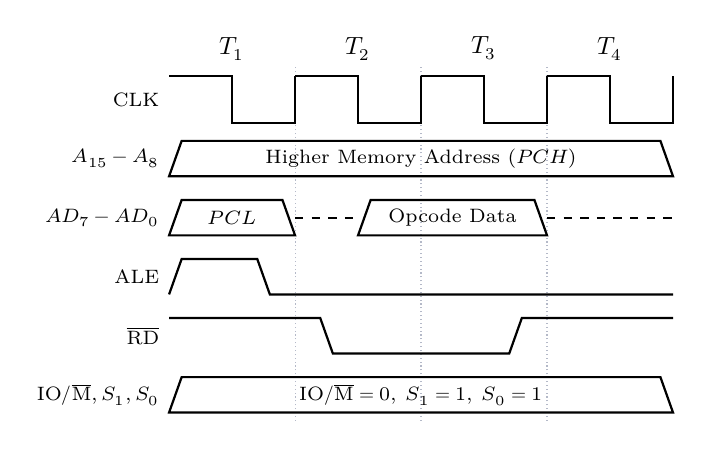
\begin{tikzpicture}[x=1.6cm, y=0.75cm, every node/.style={font=\scriptsize}]
  \foreach \boundary in {1,2,3}
    \draw[mgframe,densely dotted] (\boundary,-1.44) -- (\boundary,4.55);
  % Clock
  \node[left] at (0, 4) {CLK};
  \foreach \i in {0,1,2,3} {
    \draw[thick] (\i, 4.4) -- ++(0.5,0) -- ++(0,-0.8) -- ++(0.5,0) -- ++(0,0.8);
    \node[above, font=\small\bfseries] at (\i+0.5, 4.5) {$T_{\pgfmathparse{int(\i+1)}\pgfmathresult}$};
  }

  % A15-A8
  \node[left] at (0, 3) {$A_{15}-A_8$};
  \draw[thick] (0, 2.7) -- (0.1, 3.3) -- (3.9, 3.3) -- (4, 2.7) -- cycle;
  \node at (2, 3) {Higher Memory Address ($PCH$)};

  % AD7-AD0
  \node[left] at (0, 2) {$AD_7-AD_0$};
  \draw[thick] (0, 1.7) -- (0.1, 2.3) -- (0.9, 2.3) -- (1, 1.7) -- cycle;
  \node at (0.5, 2) {$PCL$};
  \draw[thick, dashed] (1, 2) -- (1.5, 2);
  \draw[thick] (1.5, 1.7) -- (1.6, 2.3) -- (2.9, 2.3) -- (3, 1.7) -- cycle;
  \node at (2.25, 2) {Opcode Data};
  \draw[thick, dashed] (3, 2) -- (4, 2);

  % ALE
  \node[left] at (0, 1) {ALE};
  \draw[thick] (0, 0.7) -- (0.1, 1.3) -- (0.7, 1.3) -- (0.8, 0.7) -- (4, 0.7);

  % /RD
  \node[left] at (0, 0) {$\overline{\mathrm{RD}}$};
  \draw[thick] (0, 0.3) -- (1.2, 0.3) -- (1.3, -0.3) -- (2.7, -0.3) -- (2.8, 0.3) -- (4, 0.3);

  % IO/M, S1, S0
  \node[left] at (0, -1) {$\mathrm{IO}/\overline{\mathrm{M}}, S_1, S_0$};
  \draw[thick] (0, -1.3) -- (0.1, -0.7) -- (3.9, -0.7) -- (4, -1.3) -- cycle;
  \node at (2, -1) {$\mathrm{IO}/\overline{\mathrm{M}}=0,\; S_1=1,\; S_0=1$};
\end{tikzpicture}
\end{tcolorbox}

\subsection{Memory Interfacing with 74LS138 Address Decoder}
To interface memory chips with the 8085, the address lines are partitioned into:
\begin{enumerate}[leftmargin=*]
  \item \textbf{Internal Address Lines:} Connected directly to the memory address pins to select an internal storage cell. For a chip of capacity $2^k$ bytes, $k$ address lines ($A_0$ to $A_{k-1}$) are used ($11$ lines for $2\,\mathrm{KiB}$, $12$ lines for $4\,\mathrm{KiB}$, $13$ lines for $8\,\mathrm{KiB}$).
  \item \textbf{Chip Select Decoding Lines:} High-order address lines ($A_k$ to $A_{15}$) are decoded using a decoder (such as the \textbf{74LS138 3-to-8 line decoder}) to assert the unique active-low Chip Select ($\overline{\mathrm{CS}}$) pin of the designated device.
  \item \textbf{Control Strobe Generation:} The 8085 produces $IO/\overline{M}$, $\overline{\mathrm{RD}}$, and $\overline{\mathrm{WR}}$. External logic generates $\overline{\mathrm{MEMR}} = \mathrm{OR}(IO/\overline{M}, \overline{\mathrm{RD}})$ and $\overline{\mathrm{MEMW}} = \mathrm{OR}(IO/\overline{M}, \overline{\mathrm{WR}})$.
\end{enumerate}

\begin{tcolorbox}[examplebox, title={Interfacing 4 KiB EPROM (2732) and 8 KiB RAM (6264)}]
\textbf{Design Objective:} Map a $4\,\mathrm{KiB}$ EPROM at address \texttt{0000H}--\texttt{0FFFH} and an $8\,\mathrm{KiB}$ SRAM at address \texttt{8000H}--\texttt{9FFFH}.
\par\vspace{4pt}
\begin{itemize}[leftmargin=*]
  \item \textbf{EPROM (2732, 4 KiB):} Requires $12$ address lines ($A_0-A_{11}$). Range: \texttt{0000H} to \texttt{0FFFH} ($A_{15}A_{14}A_{13}A_{12} = \mathbf{0000_2}$).
  \item \textbf{SRAM (6264, 8 KiB):} Requires $13$ address lines ($A_0-A_{12}$). Range: \texttt{8000H} to \texttt{9FFFH} ($A_{15}A_{14}A_{13} = \mathbf{100_2}$, with $A_{12}=0$ for \texttt{8000H-8FFFH} and $A_{12}=1$ for \texttt{9000H-9FFFH}).
  \item \textbf{Decoder Hookup (74LS138):}
  \begin{itemize}[leftmargin=*]
    \item Connect inputs $C, B, A$ to $A_{15}, A_{14}, A_{13}$.
    \item Set enables: $E_1 = \mathrm{GND}$, $E_2 = \mathrm{IO}/\overline{\mathrm{M}}$ (active-low memory enable), and $E_3 = +5\,\mathrm{V}$.
    \item Output $\overline{Y}_0$ ($A_{15}A_{14}A_{13} = 000_2$, with $A_{12}=0$) selects the $4\,\mathrm{KiB}$ EPROM $\overline{\mathrm{CS}}$.
    \item Output $\overline{Y}_4$ ($A_{15}A_{14}A_{13} = 100_2$) selects the $8\,\mathrm{KiB}$ RAM $\overline{\mathrm{CS}}$.
  \end{itemize}
\end{itemize}
\end{tcolorbox}

\par\vspace{6pt}\noindent
\begingroup
\setlength{\extrarowheight}{2.5pt}
\noindent\begin{tabularx}{\linewidth}{|B{3.2cm}|B{2.5cm}|B{2.5cm}|Y|}
\hline
\textbf{Device \& Capacity} & \textbf{Address Range} & \textbf{Address Lines Used} & \textbf{Decoding Logic / 74LS138 Output} \\ \hline
EPROM (2732, $4\,\mathrm{KiB}$) & \texttt{0000H}--\texttt{0FFFH} & $A_0-A_{11}$ internal & $\overline{Y}_0 = \overline{A_{15}}\,\overline{A_{14}}\,\overline{A_{13}}$ connected to EPROM $\overline{\mathrm{CE}}$ \\ \hline
SRAM (6264, $8\,\mathrm{KiB}$) & \texttt{8000H}--\texttt{9FFFH} & $A_0-A_{12}$ internal & $\overline{Y}_4 = A_{15}\,\overline{A_{14}}\,\overline{A_{13}}$ connected to SRAM $\overline{\mathrm{CE}}$ \\ \hline
Unused Address Space & \texttt{1000H}--\texttt{7FFFH}, \texttt{A000H}--\texttt{FFFFH} & --- & Available for peripheral I/O and future memory expansion. \\ \hline
\end{tabularx}\par
\endgroup

\section{Intel 8086 Architecture, Pins and Segmented Memory}

\begin{tcolorbox}[defbox, title={Intel 8086 Architectural Overview}]
The \textbf{Intel 8086} is a 16-bit H-MOS microprocessor with a 20-bit physical address bus ($1\,\mathrm{MiB}$ addressing space) and a 16-bit data bus. It divides internal operations into two autonomous processing units executing in parallel:
\begin{itemize}[leftmargin=*]
  \item \textbf{Bus Interface Unit (BIU):} Fetches instructions, handles address translation, reads and writes memory operands, and maintains a \textbf{6-byte Instruction Prefetch Queue}.
  \item \textbf{Execution Unit (EU):} Receives pre-decoded opcodes from the queue, executes instructions using the 16-bit ALU, register file, and updates status flags.
\end{itemize}
\end{tcolorbox}

\begin{tcolorbox}[tikzbox, title={Intel 8086 Functional Internal Architecture (BIU and EU)}]
\centering
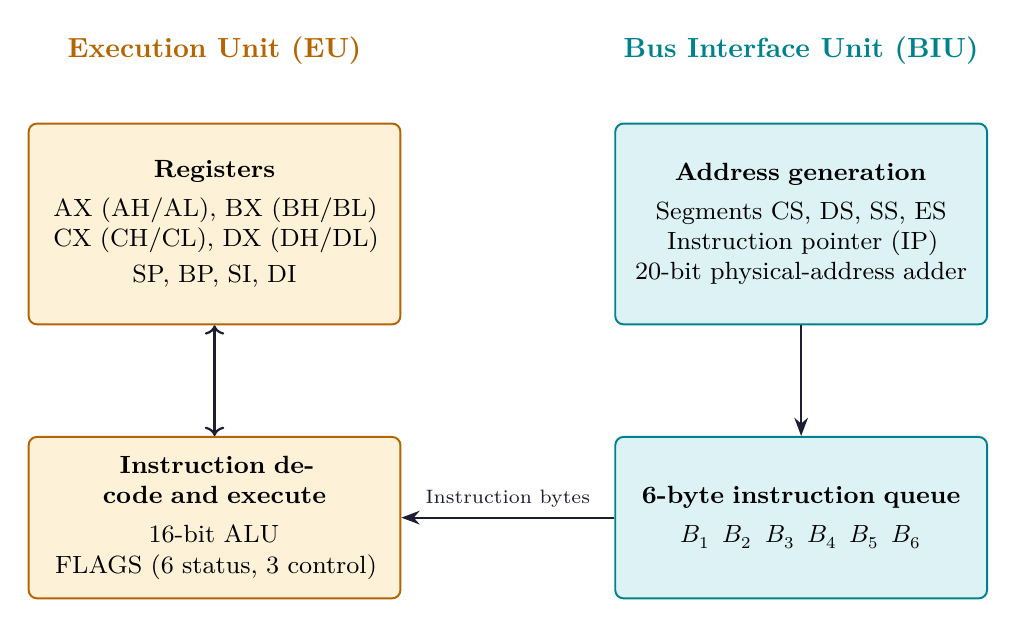
\begin{tikzpicture}[every node/.style={font=\small},
  unit/.style={align=center,text width=4.3cm,inner sep=6pt}]
  \node[font=\normalsize\bfseries,text=myamber] at (0,4.45) {Execution Unit (EU)};
  \node[font=\normalsize\bfseries,text=myteal] at (7.45,4.45) {Bus Interface Unit (BIU)};
  \node[amberblock,unit,minimum height=2.55cm] (regs) at (0,2.25)
    {\textbf{Registers}\\[3pt]
    AX (AH/AL), BX (BH/BL)\\ CX (CH/CL), DX (DH/DL)\\[2pt]
    SP, BP, SI, DI};
  \node[block,unit,minimum height=2.55cm] (seg) at (7.45,2.25)
    {\textbf{Address generation}\\[3pt]
    Segments CS, DS, SS, ES\\ Instruction pointer (IP)\\
    20-bit physical-address adder};
  \node[amberblock,unit,minimum height=2.05cm] (alu) at (0,-1.48)
    {\textbf{Instruction decode and execute}\\[3pt]
    16-bit ALU\\ FLAGS (6 status, 3 control)};
  \node[block,unit,minimum height=2.05cm] (queue) at (7.45,-1.48)
    {\textbf{6-byte instruction queue}\\[3pt]
    $B_1\enspace B_2\enspace B_3\enspace B_4\enspace B_5\enspace B_6$};
  \draw[arrow,<->,thick] (regs.south) -- (alu.north);
  \draw[arrow,thick] (seg.south) -- (queue.north);
  \draw[arrow,thick] (queue.west) -- node[above,font=\scriptsize] {Instruction bytes} (alu.east);
\end{tikzpicture}
\end{tcolorbox}

\subsection{Segmented Memory and Physical Address Generation}
Memory in the 8086 is organized as a segmented address space of $1\,\mathrm{MiB}$ ($2^{20}$ bytes), divided into logical segments of up to $64\,\mathrm{KiB}$ each. Four segments can be active concurrently:
\begin{enumerate}[leftmargin=*]
  \item \textbf{Code Segment (CS):} Contains executable instructions; addressed with Instruction Pointer ($\mathrm{IP}$).
  \item \textbf{Data Segment (DS):} Holds program data variables; default segment for general registers and strings.
  \item \textbf{Stack Segment (SS):} Stores subroutines return addresses, parameters, and stack data; addressed with $\mathrm{SP}$ and $\mathrm{BP}$.
  \item \textbf{Extra Segment (ES):} Holds alternate destination data in string instructions (addressed via $\mathrm{DI}$).
\end{enumerate}

\begin{tcolorbox}[formulabox, title={8086 Physical Address Calculation}]
The 20-bit Physical Address is generated inside the BIU by shifting the 16-bit Segment Base Address left by 4 bit positions (multiplying by $16_{10}$ or $10_{16}$) and adding the 16-bit Offset Address:
\[
\mathbf{\mathrm{Physical\ Address}} = (\mathrm{Segment\ Base} \times 10_{\mathrm{H}}) + \mathrm{Offset}
\]
\textbf{Example:} If $\mathrm{CS} = 2500_{\mathrm{H}}$ and $\mathrm{IP} = 0128_{\mathrm{H}}$:
\[
\mathrm{Shifted\ Base} = 25000_{\mathrm{H}}, \quad \mathrm{Physical\ Address} = 25000_{\mathrm{H}} + 0128_{\mathrm{H}} = \mathbf{25128_{\mathrm{H}}}
\]
\end{tcolorbox}

\subsection{Memory Banking: Odd and Even Banks}
The $1\,\mathrm{MiB}$ physical memory is physically structured as two parallel $512\,\mathrm{KiB}$ banks to support both 8-bit and 16-bit transfers in a single bus cycle:
\begin{itemize}[leftmargin=*]
  \item \textbf{Even Bank (Lower Bank):} Stores even-addressed bytes ($00000_{\mathrm{H}}, 00002_{\mathrm{H}}, \dots$). Connected to lower data lines $D_0-D_7$. Enabled when address line $\mathbf{A_0 = 0}$.
  \item \textbf{Odd Bank (Higher Bank):} Stores odd-addressed bytes ($00001_{\mathrm{H}}, 00003_{\mathrm{H}}, \dots$). Connected to upper data lines $D_8-D_{15}$. Enabled when Bus High Enable $\mathbf{\overline{BHE} = 0}$.
\end{itemize}

\par\vspace{6pt}\noindent
\begingroup
\setlength{\extrarowheight}{2.5pt}
\noindent\begin{tabularx}{\linewidth}{|B{2.2cm}|B{2.2cm}|B{3.2cm}|Y|}
\hline
$\mathbf{\overline{BHE}}$ & $\mathbf{A_0}$ & \textbf{Data Transfer Type} & \textbf{Bus Operation Characteristics} \\ \hline
$0$ & $0$ & Whole Word ($16$-bit) & Transfers 16-bit word at an even address in $1$ bus cycle ($D_0-D_{15}$). \\ \hline
$0$ & $1$ & Odd Byte ($8$-bit) & Transfers single byte from odd address in $1$ bus cycle via $D_8-D_{15}$. \\ \hline
$1$ & $0$ & Even Byte ($8$-bit) & Transfers single byte from even address in $1$ bus cycle via $D_0-D_7$. \\ \hline
$1$ & $1$ & None (Inactive) & Both banks disabled. \\ \hline
\end{tabularx}\par
\endgroup

\begin{tcolorbox}[examplebox, title={Aligned vs. Misaligned Word Access Penalty}]
\begin{itemize}[leftmargin=*]
  \item \textbf{Aligned Word (Even Address, e.g., \texttt{2000H}):} $A_0=0$ and $\overline{\mathrm{BHE}}=0$. Both banks respond simultaneously. Transferred in strictly \textbf{1 bus cycle} ($4$ T-states).
  \item \textbf{Misaligned Word (Odd Address, e.g., \texttt{2001H}):}
  \begin{itemize}[leftmargin=*]
    \item \textit{Cycle 1:} Read byte from odd bank at \texttt{2001H} ($A_0=1, \overline{\mathrm{BHE}}=0$ on $D_8-D_{15}$).
    \item \textit{Cycle 2:} Read byte from even bank at \texttt{2002H} ($A_0=0, \overline{\mathrm{BHE}}=1$ on $D_0-D_7$).
    \item Requires \textbf{2 consecutive bus cycles} ($8$ T-states), incurring a $100\%$ bus execution penalty.
  \end{itemize}
\end{itemize}
\end{tcolorbox}

\subsection{Minimum Mode vs. Maximum Mode Operation}
The 8086 operates in two distinct electrical modes selected by pin 33 ($\mathrm{MN}/\overline{\mathrm{MX}}$):
\par\vspace{4pt}\noindent
\begingroup
\setlength{\extrarowheight}{2pt}
\begingroup
\setlength{\LTleft}{0pt}
\setlength{\LTright}{0pt}
\begin{longtable}{|B{3.0cm}|>{\small\raggedright\arraybackslash}m{\dimexpr(\linewidth-3.0cm-6\tabcolsep-4\arrayrulewidth)/2\relax}|>{\small\raggedright\arraybackslash}m{\dimexpr(\linewidth-3.0cm-6\tabcolsep-4\arrayrulewidth)/2\relax}|}
\hline
\textbf{Parameter} & \textbf{Minimum Mode ($\mathrm{MN}/\overline{\mathrm{MX}} = V_{CC}$)} & \textbf{Maximum Mode ($\mathrm{MN}/\overline{\mathrm{MX}} = \mathrm{GND}$)} \\ \hline
\endfirsthead
\hline
\textbf{Parameter} & \textbf{Minimum Mode ($\mathrm{MN}/\overline{\mathrm{MX}} = V_{CC}$)} & \textbf{Maximum Mode ($\mathrm{MN}/\overline{\mathrm{MX}} = \mathrm{GND}$)} \\ \hline
\endhead
Target System & Single-processor standalone configuration & Multiprocessor / coprocessor configuration (8086 + 8087) \\ \hline
Control Generation & 8086 directly outputs $\overline{\mathrm{RD}}, \overline{\mathrm{WR}}, \mathrm{M}/\overline{\mathrm{IO}}, \mathrm{ALE}$ & External 8288 Bus Controller decodes status $\overline{S}_0-\overline{S}_2$ \\ \hline
Bus Arbitration & Driven by $\mathrm{HOLD}$ and $\mathrm{HLDA}$ pins & Driven by $\overline{\mathrm{RQ}}/\overline{\mathrm{GT}}_0$ and $\overline{\mathrm{RQ}}/\overline{\mathrm{GT}}_1$ request/grant lines \\ \hline
Queue Status Lines & Not available (control pins active) & Pins 24, 25 provide Queue Status ($\mathrm{QS}_0, \mathrm{QS}_1$) to 8087 \\ \hline
\end{longtable}
\endgroup\par
\endgroup

\section{Concepts of Interrupts and Direct Memory Access (DMA)}

\subsection{8085 Interrupt System and SIM/RIM Bit Architectures}
The 8085 supports 5 hardware interrupt pins with the following fixed priority order:
\par\vspace{6pt}\noindent
\begingroup
\setlength{\extrarowheight}{2.5pt}
\noindent\begin{tabularx}{\linewidth}{|B{2.2cm}|B{2.0cm}|B{2.6cm}|B{2.4cm}|Y|}
\hline
\textbf{Interrupt} & \textbf{Priority} & \textbf{Triggering Type} & \textbf{Vector Address} & \textbf{Maskability} \\ \hline
TRAP & 1 (Highest) & Edge \& Level sensitive & $0024_{\mathrm{H}}$ ($4.5 \times 8$) & Non-Maskable (cannot be disabled). \\ \hline
RST 7.5 & 2 & Rising edge sensitive & $003C_{\mathrm{H}}$ ($7.5 \times 8$) & Maskable via `SIM` instruction. \\ \hline
RST 6.5 & 3 & High-level sensitive & $0034_{\mathrm{H}}$ ($6.5 \times 8$) & Maskable via `SIM` instruction. \\ \hline
RST 5.5 & 4 & High-level sensitive & $002C_{\mathrm{H}}$ ($5.5 \times 8$) & Maskable via `SIM` instruction. \\ \hline
INTR & 5 (Lowest) & High-level sensitive & Non-vectored & Maskable via `EI` / `DI` instructions. \\ \hline
\end{tabularx}\par
\endgroup

\begin{tcolorbox}[formulabox, title={8085 SIM and RIM Instruction Bit Definitions}]
\textbf{1. Set Interrupt Mask (SIM) Format:} Configures masks and serial output line SOD.
\par\vspace{4pt}
\centering
\begin{tabular}{|c|c|c|c|c|c|c|c|}
\hline
$D_7$ & $D_6$ & $D_5$ & $D_4$ & $D_3$ & $D_2$ & $D_1$ & $D_0$ \\ \hline
\textbf{SOD} & \textbf{SOE} & \textbf{X} & \textbf{R7.5} & \textbf{MSE} & \textbf{M7.5} & \textbf{M6.5} & \textbf{M5.5} \\ \hline
\end{tabular}
\par\vspace{4pt}\raggedright
\begin{itemize}[leftmargin=*, itemsep=1pt]
  \item \textbf{SOD:} Serial Output Data to be latched into SOD pin.
  \item \textbf{SOE:} Serial Output Enable ($1 = \text{enable SOD latch}$; $0 = \text{disable}$).
  \item \textbf{R7.5:} Reset RST 7.5 flip-flop ($1 = \text{clear edge latch}$).
  \item \textbf{MSE:} Mask Set Enable ($1 = \text{load M7.5, M6.5, M5.5}$; $0 = \text{ignore mask bits}$).
  \item \textbf{M7.5, M6.5, M5.5:} Individual interrupt masks ($1 = \text{masked/disabled}$; $0 = \text{unmasked/available}$).
\end{itemize}
\par\vspace{6pt}
\textbf{2. Read Interrupt Mask (RIM) Format:} Reads masks, pending interrupts, and SID pin.
\par\vspace{4pt}
\centering
\begin{tabular}{|c|c|c|c|c|c|c|c|}
\hline
$D_7$ & $D_6$ & $D_5$ & $D_4$ & $D_3$ & $D_2$ & $D_1$ & $D_0$ \\ \hline
\textbf{SID} & \textbf{I7.5} & \textbf{I6.5} & \textbf{I5.5} & \textbf{IE} & \textbf{M7.5} & \textbf{M6.5} & \textbf{M5.5} \\ \hline
\end{tabular}
\par\vspace{4pt}\raggedright
\begin{itemize}[leftmargin=*, itemsep=1pt]
  \item \textbf{SID:} Current digital logic level on Serial Input Data pin.
  \item \textbf{I7.5, I6.5, I5.5:} Pending interrupt flags ($1 = \text{interrupt request is pending execution}$).
  \item \textbf{IE:} Interrupt Enable status flag ($1 = \text{interrupts globally enabled by `EI`}$).
  \item \textbf{M7.5, M6.5, M5.5:} Current mask status of RST interrupts.
\end{itemize}
\end{tcolorbox}

\subsection{8086 Interrupt Vector Table (IVT)}
The 8086 allocates the lowest $1\,\mathrm{KiB}$ of physical memory (\texttt{00000H}--\texttt{003FFH}) as the \textbf{Interrupt Vector Table (IVT)}. It supports up to 256 interrupts (Types $0$ to $255$):
\begin{itemize}[leftmargin=*]
  \item Each vector entry consumes \textbf{4 bytes}: 2 bytes for the Interrupt Service Routine (ISR) Instruction Pointer ($\mathrm{IP}$) and 2 bytes for the Code Segment ($\mathrm{CS}$).
  \item Physical address of vector type $N$:
  \[
  \mathbf{\mathrm{Base\ Address}} = 4 \times N
  \]
  \item Dedicated Predefined Interrupts:
  \begin{itemize}[leftmargin=*]
    \item \textbf{Type 0:} Divide by Zero error (fault).
    \item \textbf{Type 1:} Single-Step Trap (enabled when Trap Flag $\mathrm{TF}=1$).
    \item \textbf{Type 2:} Non-Maskable Interrupt ($\mathrm{NMI}$ pin).
    \item \textbf{Type 3:} 1-byte Breakpoint instruction (`INT 3`).
    \item \textbf{Type 4:} Overflow exception (`INTO` instruction when Overflow Flag $\mathrm{OF}=1$).
  \end{itemize}
\end{itemize}

\subsection{Direct Memory Access (DMA)}
\begin{tcolorbox}[defbox, title={Direct Memory Access (DMA) Principle}]
\textbf{Direct Memory Access (DMA)} is a high-speed data transfer mechanism wherein external high-bandwidth peripherals (hard disks, network controllers) exchange data directly with system RAM without CPU intervention. A dedicated hardware peripheral—the \textbf{DMA Controller (DMAC, e.g., Intel 8257/8237)}—acts as an alternate bus master.
\end{tcolorbox}

\begin{itemize}[leftmargin=*]
  \item \textbf{Bus Handshake Sequence:}
  \begin{enumerate}[leftmargin=*]
    \item Peripheral asserts DMA Request ($\mathrm{DRQ}$) to DMAC.
    \item DMAC asserts $\mathrm{HOLD}$ pin to the 8085/8086.
    \item CPU finishes current bus cycle, floats its address, data, and control lines into high impedance, and asserts Hold Acknowledge ($\mathrm{HLDA}$).
    \item DMAC asserts DMA Acknowledge ($\mathrm{DACK}$) to the peripheral, drives the memory address bus, and strobes $\overline{\mathrm{IOR}}$ and $\overline{\mathrm{MEMW}}$ (or $\overline{\mathrm{MEMR}}$ and $\overline{\mathrm{IOW}}$) simultaneously to transfer data in a single clock cycle.
    \item When the block transfer completes, DMAC lowers $\mathrm{HOLD}$, and CPU resumes normal bus control.
  \end{enumerate}
  \item \textbf{DMA Transfer Modes:}
  \begin{itemize}[leftmargin=*]
    \item \textit{Burst Mode (Block Transfer):} DMAC retains the bus continuously until the entire data buffer is transferred. Fast, but locks out the CPU.
    \item \textit{Cycle Stealing Mode:} DMAC transfers one byte per request, releasing the bus between bytes so the CPU is not starved.
  \end{itemize}
\end{itemize}

\section{Instruction Sets and Addressing Modes}

\subsection{Addressing Modes of 8085 and 8086}
\par\vspace{6pt}\noindent
\begingroup
\setlength{\extrarowheight}{2.5pt}
\noindent\begin{tabularx}{\linewidth}{|B{3.2cm}|B{3.4cm}|Y|}
\hline
\textbf{Addressing Mode} & \textbf{8085 Example \& Syntax} & \textbf{8086 Example \& Syntax} \\ \hline
Immediate & `MVI A, 45H` ($A \leftarrow 45_{\mathrm{H}}$) & `MOV AX, 1234H` ($AX \leftarrow 1234_{\mathrm{H}}$) \\ \hline
Register & `MOV A, B` ($A \leftarrow B$) & `MOV CX, DX` ($CX \leftarrow DX$) \\ \hline
Direct & `LDA 2050H` ($A \leftarrow [2050_{\mathrm{H}}]$) & `MOV AX, [2050H]` ($AX \leftarrow [DS \times 16 + 2050_{\mathrm{H}}]$) \\ \hline
Register Indirect & `MOV A, M` ($A \leftarrow [HL]$) & `MOV AX, [BX]` ($AX \leftarrow [DS \times 16 + BX]$) \\ \hline
Based & \textit{Not available} & `MOV AX, [BX + 04H]` ($AX \leftarrow [DS \times 16 + BX + 4]$) \\ \hline
Indexed & \textit{Not available} & `MOV AX, [SI + 08H]` ($AX \leftarrow [DS \times 16 + SI + 8]$) \\ \hline
Based-Indexed & \textit{Not available} & `MOV AX, [BX + DI + 10H]` \\ \hline
Implied / Implicit & `CMA` (Complement Accumulator) & `STC` (Set Carry Flag) \\ \hline
\end{tabularx}\par
\endgroup

\subsection{Key Assembly Programs with Derivations}

\begin{tcolorbox}[examplebox, title={8085 BCD Addition with DAA Instruction}]
\textbf{Problem:} Add two Packed BCD numbers stored at memory locations \texttt{2050H} ($= 48_{\mathrm{H}}$) and \texttt{2051H} ($= 37_{\mathrm{H}}$), and store the resulting BCD sum ($= 85_{\mathrm{H}}$) at \texttt{2052H}.
\begin{verbatim}
        LDA  2050H      ; Load first BCD operand into Accumulator (A = 48H)
        MOV  B, A       ; Move to register B
        LDA  2051H      ; Load second BCD operand (A = 37H)
        ADD  B          ; Binary addition: 48H + 37H = 7FH (AC = 0, CY = 0)
        DAA             ; Decimal Adjust: lower nibble 0FH > 9, adds 06H:
                        ; 7FH + 06H = 85H (Auxiliary carry set, CY = 0)
        STA  2052H      ; Store unpacked BCD result 85H at 2052H
        HLT             ; Terminate program
\end{verbatim}
\textbf{DAA Rule:} If the lower nibble $> 9$ or $AC = 1$, add $06_{\mathrm{H}}$ to Accumulator. If upper nibble $> 9$ or $CY = 1$, add $60_{\mathrm{H}}$ to Accumulator.
\end{tcolorbox}

\begin{tcolorbox}[examplebox, title={8086 Block Copy Using String Primitives}]
\textbf{Problem:} Copy a 128-byte block from source address \texttt{DS:0100H} to destination address \texttt{ES:0200H}.
\begin{verbatim}
        MOV  AX, 2000H  ; Segment base address
        MOV  DS, AX     ; Initialize Data Segment
        MOV  ES, AX     ; Initialize Extra Segment
        MOV  SI, 0100H  ; SI points to Source Offset
        MOV  DI, 0200H  ; DI points to Destination Offset
        MOV  CX, 0080H  ; CX = 128 bytes counter
        CLD             ; Clear Direction Flag (DF = 0, auto-increment SI and DI)
        REP  MOVSB      ; Repeat MOVSB while CX != 0:
                        ; [ES:DI] <- [DS:SI], SI <- SI+1, DI <- DI+1, CX <- CX-1
        HLT
\end{verbatim}
\end{tcolorbox}

\subsection{Subroutine CALL and RET Stack Operations}
Both 8085 and 8086 use the hardware stack for subroutine execution and interrupt handling:
\begin{itemize}[leftmargin=*]
  \item \textbf{8085 CALL / RET:} \texttt{CALL addr} decrements $\mathrm{SP}$ by 2 and pushes the 16-bit return address onto the stack ($[\mathrm{SP}-1] \leftarrow \mathrm{PCH}$, $[\mathrm{SP}-2] \leftarrow \mathrm{PCL}$, $\mathrm{SP} \leftarrow \mathrm{SP}-2$). \texttt{RET} pops the top two stack bytes into $\mathrm{PC}$ ($\mathrm{PCL} \leftarrow [\mathrm{SP}]$, $\mathrm{PCH} \leftarrow [\mathrm{SP}+1]$, $\mathrm{SP} \leftarrow \mathrm{SP}+2$).
  \item \textbf{8086 Near vs. Far CALL:}
  \begin{itemize}[leftmargin=*]
    \item \textit{Near CALL (Intra-Segment):} Target resides within the current Code Segment. Only 16-bit $\mathrm{IP}$ is pushed onto stack ($\mathrm{SP} \leftarrow \mathrm{SP}-2$).
    \item \textit{Far CALL (Inter-Segment):} Target resides in a different segment. Both $\mathrm{CS}$ and $\mathrm{IP}$ are pushed onto the stack ($4$ bytes total), and new base/offset values are loaded.
  \end{itemize}
  \item \textbf{Hardware Multiplication and Division in 8086:}
  Unlike the 8085, the 8086 provides native integer multiplication (\texttt{MUL}, \texttt{IMUL}) and division (\texttt{DIV}, \texttt{IDIV}). For 8-bit operations: $\mathrm{AX} \leftarrow \mathrm{AL} \times r/m8$; for 16-bit operations: $(\mathrm{DX}:\mathrm{AX}) \leftarrow \mathrm{AX} \times r/m16$.
\end{itemize}

\begingroup
\par\smallskip\noindent \textbf{Comprehensive Comparison: Intel 8085 vs. Intel 8086}\par\nobreak
\par\vspace{5pt}
\begingroup
\setlength{\extrarowheight}{2.5pt}
\begingroup
\setlength{\LTleft}{0pt}
\setlength{\LTright}{0pt}
\begin{longtable}{|B{3.2cm}|>{\small\raggedright\arraybackslash}m{\dimexpr(\linewidth-3.2cm-6\tabcolsep-4\arrayrulewidth)/2\relax}|>{\small\raggedright\arraybackslash}m{\dimexpr(\linewidth-3.2cm-6\tabcolsep-4\arrayrulewidth)/2\relax}|}
\hline
\textbf{Architectural Feature} & \textbf{Intel 8085} & \textbf{Intel 8086} \\ \hline
\endfirsthead
\hline
\textbf{Architectural Feature} & \textbf{Intel 8085} & \textbf{Intel 8086} \\ \hline
\endhead
Data Bus Width & 8 bits & 16 bits \\ \hline
Address Bus Width & 16 bits ($64\,\mathrm{KiB}$ address space) & 20 bits ($1\,\mathrm{MiB}$ address space) \\ \hline
Operating Frequency & $3.072\,\mathrm{MHz}$ (standard) & $5\,\mathrm{MHz}, 8\,\mathrm{MHz}, 10\,\mathrm{MHz}$ \\ \hline
Internal Architecture & Single functional processing unit & Split into BIU and EU (Pipelined) \\ \hline
Instruction Queue & None & 6-byte FIFO prefetch queue \\ \hline
Memory Organization & Single linear $64\,\mathrm{KiB}$ space & Segmented ($4 \times 64\,\mathrm{KiB}$ active banks) \\ \hline
Memory Banking & None & Two $512\,\mathrm{KiB}$ banks (Even and Odd) \\ \hline
Operating Modes & Single fixed operating mode & Minimum Mode and Maximum Mode \\ \hline
Interrupt Vectoring & Vector table shared with RAM & Dedicated $1\,\mathrm{KiB}$ IVT ($256$ vectors) \\ \hline
Multiply and divide & Not supported in hardware & Hardware `MUL` and `DIV` instructions \\ \hline
\end{longtable}
\endgroup\par
\endgroup
\endgroup

\newpage
% ─── Quick Revision Section ────────────────────────────────────────────────────
\begin{center}
  {\large\bfseries\color{myred} Quick Revision --- Module 1}\\[3pt]
  {\small\color{mydark} 8085 and 8086 Microprocessor Systems $|$ EC403}
\end{center}
\noindent{\color{myred}\rule{\linewidth}{1.2pt}}\vspace{4pt}

\begin{tcolorbox}[formulabox, title={Key Formulas at a Glance}]
\renewcommand{\arraystretch}{1.2}
\noindent\begin{tabularx}{\linewidth}{B{4.5cm}Y}
Memory Capacity & $\text{Capacity} = 2^n \text{ bytes}$, where $n$ is the number of address bus lines. \\
T-State Period & $T = 1 / f_{CLK} = 1 / 3.072\,\mathrm{MHz} \approx 325.5\,\mathrm{ns}$ (for 8085). \\
8086 Physical Address & $\text{Physical Address} = (\text{Segment Register} \times 16_{10}) + \text{Offset Address}$. \\
8086 IVT Pointer Address & $\text{Vector Pointer Address} = 4 \times N$ (where $N = 0, 1, \dots, 255$ is Interrupt Type). \\
Bank Selection & Even Bank: $A_0 = 0$; Odd Bank: $\overline{\mathrm{BHE}} = 0$. Word access on even boundary takes 1 cycle. \\
\end{tabularx}\par
\end{tcolorbox}

\begin{tcolorbox}[defbox, title={One-Line Definitions}]
\begin{itemize}[leftmargin=*, itemsep=2pt]
  \item \textbf{Microprocessor:} Programmable, clock-driven VLSI IC containing CPU registers, ALU, and control unit.
  \item \textbf{ALE (Address Latch Enable):} Active-high pulse generated during $T_1$ to latch lower multiplexed address bits ($AD_0-AD_7$).
  \item \textbf{T-State:} One basic subdivision of a machine cycle corresponding to exactly one complete clock period.
  \item \textbf{Machine Cycle:} Time required by the CPU to execute one discrete bus operation (Fetch, Read, Write).
  \item \textbf{Pipelining (8086):} Overlapping technique where BIU prefetches instructions into a 6-byte queue while EU executes.
  \item \textbf{Bus High Enable ($\overline{\mathrm{BHE}}$):} Active-low control signal enabling data transfer over upper data bus lines ($D_8-D_{15}$).
  \item \textbf{TRAP:} Highest-priority non-maskable, edge-and-level sensitive vectored interrupt of the 8085 ($0024_{\mathrm{H}}$).
  \item \textbf{DMA (Direct Memory Access):} High-speed hardware data transfer managed directly by a DMAC without CPU intervention.
\end{itemize}
\end{tcolorbox}

\begin{tcolorbox}[exambox, title={Frequently Asked / Viva Questions}]
\begin{enumerate}[leftmargin=*, label=\textbf{Q\arabic*.}, itemsep=3.5pt]
  \item \Q{Why are AD0--AD7 multiplexed in 8085?}
  To minimize the physical package pin count to 40 pins while providing separate address and data paths using external transparent latches (74LS373) strobed by ALE.
  \item \Q{What is the difference between instruction cycle, machine cycle, and T-state?}
  An Instruction Cycle is the total time to fetch and execute an instruction ($1-5$ Machine Cycles); each Machine Cycle is a discrete bus operation ($3-6$ T-States); a T-state is one clock period.
  \item \Q{Why does Opcode Fetch require 4 T-states while Memory Read requires only 3?}
  The extra fourth state ($T_4$) is required for internal decoding and machine encoding of the fetched instruction byte inside the CPU.
  \item \Q{What are the functions of IO/M, S1, and S0 pins in 8085?}
  They indicate bus status: $\mathrm{IO}/\overline{\mathrm{M}}$ distinguishes memory ($0$) from I/O ($1$); $S_1, S_0$ identify Fetch ($1,1$), Read ($1,0$), Write ($0,1$), and Halt ($0,0$).
  \item \Q{Explain the role of the 8086 Bus Interface Unit (BIU) and Execution Unit (EU).}
  BIU handles bus operations, address computation, and prefetches 6 instruction bytes into a FIFO queue. EU decodes and executes instructions via the 16-bit ALU.
  \item \Q{Why is memory segmented in 8086 and how is physical address calculated?}
  Segmentation allows a 16-bit processor to address $1\,\mathrm{MiB}$ with 16-bit registers and provides code relocation. Physical address is calculated as $(\mathrm{Segment\ Base} \times 16_{10}) + \mathrm{Offset}$.
  \item \Q{What is the penalty of accessing a 16-bit word at an odd address in 8086?}
  It requires two consecutive bus cycles ($8$ T-states) instead of one ($4$ T-states) because the two bytes reside in different memory banks (Even and Odd banks).
  \item \Q{What is the purpose of the 8288 Bus Controller in 8086 Maximum Mode?}
  In maximum mode, the 8086 floats its control pins; the 8288 decodes status outputs $\overline{S}_2\overline{S}_1\overline{S}_0$ to generate system bus strobes ($\overline{\mathrm{MRDC}}, \overline{\mathrm{MWTC}}, \overline{\mathrm{IORC}}, \overline{\mathrm{IOWC}}$).
  \item \Q{How does the 8085 handle priority among interrupts and what do SIM/RIM do?}
  Hardware priority is fixed: $\mathrm{TRAP} > \mathrm{RST\,7.5} > \mathrm{RST\,6.5} > \mathrm{RST\,5.5} > \mathrm{INTR}$. `SIM` sets interrupt masks and serial output (SOD); `RIM` reads pending flags and serial input (SID).
  \item \Q{What happens during HOLD and HLDA signals during DMA?}
  An external DMAC asserts $\mathrm{HOLD}$; the CPU finishes its current cycle, floats address, data, and control lines into high impedance, and returns $\mathrm{HLDA}$ to grant bus mastership.
\end{enumerate}
\end{tcolorbox}

\end{document}
